\documentclass{beamer}

\year=2023
\month=7
\day=11

\usetheme{simple}
\setbeamertemplate{items}[circle]
\setbeamertemplate{section in toc}[sections numbered]
\setbeamerfont{footnote}{size=\scriptsize}
\def\bibfont{\tiny}
\usepackage{lmodern}
\usepackage[scale=2]{ccicons}

\title{Detección de noticias falsas usando Procesado de Lenguaje Natural}
% \subtitle{Trabajo de Fin de Grado}
\date{\today}
\author{Miguel Ricardo Claramunt Argote}
\institute{Escola Tècnica Superior d'Enginyeria -- Universitat de València}

\begin{document}

\setwatermark[hoffset=0.02\textwidth,voffset=0.02\textwidth]{\includesvg[width=0.7\textwidth]{img/ETSE_2_linies.svg}}
% Title page frame
\begin{frame}
    \titlepage 
\end{frame}

\setwatermark[voffset=0.03\textwidth]{\includesvg[height=0.06\textwidth]{img/ETSE_icono.svg}}

% Outline frame
\begin{frame}{Esquema de la presentación}
    \tableofcontents
\end{frame}

\section{Introducción}
\begin{frame}{1.1. Introducción}

Las \textit{fake news} son piezas de texto con estilo pseudoperiodístico que tienen como objetivo desinformar a los lectores.

% \vspace{2ex}

% Estas `noticias' toman relevancia mundial en las elecciones presidenciales de E.E.U.U. en 2016, superando en \textit{engagement} a los medios tradicionales.

\vspace{2ex}

Motivos principales que incentivan la difusión de \textit{fake news}:
\begin{itemize}
    \item \underline{\smash{Económico:}} publicidad en la página web.
    % y el tráfico que generan estos sitios, pueden generar hasta 30.000 \$ mensuales.\footnote{\citep{Sydell2016}}
    \item \underline{\smash{Ideológico:}} apoyo de una agenda política.\footnote{\citep{AlcottGentzkow2017, Sydell2016}}
    % las \textit{fake news} consiguen enturbiar la opinión pública para apoyar una agenda política determinada.
\end{itemize}

\end{frame}

\begin{frame}{1.2. Motivación}

\textit{Fact checking}:
\begin{itemize}
    \item Exhaustivo, laborioso.
    \item Mayoritariamente manual.
    \item Grandes beneficios si se automatiza: \textit{LLMs}.
\end{itemize}

% Las redes sociales han transformado todo el proceso: formato, difusión, `viralidad', \textit{bots}, etc.

% \end{frame}

% \begin{frame}{Motivación}

% Las \textit{fake news}: 
% manipulan la percepción de la realidad, generando desconfianza y conflicto social.\footnote{\citep{CITSa}}

% % \vspace{2ex}

% El \textit{fact checking} es un proceso muy exhaustivo, laborioso y prácticamente manual, por lo se beneficiaría de la automatización.

\vspace{1ex}

% Los \textit{Large Language Models} (LLMs) permiten desarrollar aplicaciones para automatizar partes de este proceso.

% las siguientes aplicaciones: clasificador de noticias verdaderas/falsas, \textit{Information Retrieval}, resumen automático.

\vspace{2ex}

Otros beneficios: reducción de prejuicios en colectivos minorizados, mejora de la imagen del periodismo/periodista, etc.

\end{frame}

\begin{frame}{1.3. Objetivos}

Objetivo principal:
\begin{itemize}
    \item Desarrollar una solución que permita detectar noticias falsas.
    \begin{itemize}
        \item Clasificación a partir de características estilísticas.
        \item Estudio comparativo: cantidad/calidad de información, arquitectura/tamaño de los modelos. 
    \end{itemize}
\end{itemize}

\vspace{2ex}

Objetivos transversales:
\begin{itemize}
    \item Definición del término de \textit{fake news} y discutir las implicaciones en nuestro trabajo.
    \item Conocer en profundidad cómo funcionan los modelos y los sesgos implícitos.
    \item Aplicación de técnicas de \textit{Explanable AI} (XAI) para intentar entender el `razonamiento' de los modelos.
    % \item Conocer los sesgos de los modelos y cómo afectan la arquitectura y el aprendizaje en estos.
\end{itemize}

\end{frame}

\section{Definiciones}
\begin{frame}{2. Definiciones y área de estudio}

% Diferentes formulaciones del concepto aplicadas a noticias \citep{AlcottGentzkow2017,Lazer2018}.

% \vspace{2ex}

% \citet{Mourao2019} encuentran que la mayoría de información que se difunde no sigue la estructura de una noticia, por lo que hace falta reformular el concepto.

% \vspace{2ex}

% A partir del trabajo de , utilizamos la siguiente definición:

% \vspace{2ex}

\begin{quotation}
    \underline{Disinformation (Desinformación).} Contenido proposicional de signos que tergiversa el estado del mundo con la intención de engañar. --- \citep{Khan2021}   
\end{quotation}

\vspace{2ex}

Problema complejo, límite del area de aplicación a noticias:
\begin{itemize}
    \item \underline{\smash{Recopilables:}} gran disponibilidad de BBDD.
    \item \underline{\smash{Categorizables:}} aprendizaje supervisado.
\end{itemize}

% Ya que el problema es complejo, limitamos el área de aplicación a noticia, que son fácilmente recopilables y categorizables, ayudando al entrenamiento supervisado de los modelos.

\end{frame}

\section{Estado del arte}
\begin{frame}{3. Antecedentes y tecnologías}

% El problema no se conceptualizó hasta la publicación de los trabajos de \citet{Cohen2011, Flew2012}, motivado por los avances en el procesado del lenguaje natural, bases de datos e \textit{information retrieval} de la época.

Se han desarrollado dos enfoques para abordar este problema:
\begin{itemize}
    \item \underline{\smash{Basado en patrones:}}  estilo o sintaxis, métricas de RRSS, minería de datos enfocada a emociones.
    \item \underline{\smash{Basado en evidencias.}} similaridad semántica entre \textit{claim} y evidencia.
\end{itemize} 

\vspace{2ex}

Trabajos relevantes: 
\begin{itemize}
    \item DeClarE \citep{Popat2018}
    \item HAN \citep{Ma2019}
    \item GET \citep{Xu2022}
\end{itemize}

\end{frame}

% \begin{frame}{Tecnologías}

% \textbf{DeClarE \citep{Popat2018}.} Basado en evidencias, utiliza redes neuronales convolucionales (CNN) para extraer características locales de las evidencias y contraevidencias; mientras que usa redes recurrentes (RNN) para capturar dependencias entre diferentes evidencias.


% \textbf{HAN \citep{Ma2019}.} Basado en patrones, extrae las \textit{features} mediante una \textit{Hierarchical Attention Network} (HAN) que extrae relaciones a nivel de palabra y a nivel de oración.

% \vspace{4ex}

% \textbf{GET \citep{Xu2022}.} Unifica los dos enfoques y propone una solución utilizando grafos, que permiten capturar dependencias semánticas a larga distancia.

% \end{frame}

\section{Análisis del problema}
\begin{frame}{4.1. \textit{Claim} y evidencia}
\begin{itemize}
    \item \textit{Claim}: equivalente al titular de una noticia, pieza de información a verificar.
    \item Evidencia: hecho, dato o información que apoya o refuta la \textit{claim}.
\end{itemize}
\end{frame}

\begin{frame}{4.2. Dataset: Politifact\footnote{\citep{Popat2017}} y Snopes\footnote{\citep{Vlachos2014}}}

Un \textit{claim} y varias evidencias por noticia. 

\vspace{0.5ex}

Creación de dos datasets, {P-S}\textsubscript{One} y {P-S}\textsubscript{All}:
\begin{itemize}
    \item {P-S}\textsubscript{One}: una \textit{claim}, una evidencia elegida aleatoriamente.
    \item {P-S}\textsubscript{All}: una \textit{claim}, todas las evidencias.
\end{itemize}

% \vspace{1ex}

% {P-S}\textsubscript{One} y {P-S}\textsubscript{All}; el primero tendrá, para cada \textit{claim}, una evidencia elegida aleatoriamente; el segundo las tendrá todas.

% \vspace{1ex}

% Existe un pequeño desbalanceo (3:2); no aplicamos ninguna técnica de \textit{Data Augmentation} debido a que no es tan exagerado.

\vspace{2ex}

% \begin{frame}
\begin{table}
    \hfill
    \begin{tabular}{ccrr}
        \hline
        \textbf{Dataset} & \textbf{Etiqueta} & \textbf{\#} & \textbf{\#} \\\hline
        \multirow{2}{*}{PolitiFact} & True & 186 & \multirow{2}{*}{356} \\
         & False & 170 &  \\ \hline
        \multirow{2}{*}{Snopes} & True & 116 & \multirow{2}{*}{433} \\
         & False & 317 & \\\hline
    \end{tabular}
    % \caption{Conteo de muestras.}
    % \label{tab:sp-new}
    \hfill
    \begin{tabular}{cr}
        \hline
        \textbf{Estadístico} & \multicolumn{1}{c}{\textbf{Valor}} \\ \hline
        $\mu$ & 7,43 \\
        $\sigma$ & 6,34 \\
        Mín. & 1 \\
        \text{Q}\textsubscript{1} & 2 \\
        \text{Q}\textsubscript{2} & 5 \\
        \text{Q}\textsubscript{3} & 11 \\
        Máx. & 27 \\\hline
    \end{tabular}
    % \label{tab:sp-stats}
    \hfill\null
    \caption{Conteo de muestras y estadísticos de longitud de noticias.}
\end{table}
% \end{frame}

\end{frame}

\begin{frame}{4.3. Dataset: News\footnote{\citep{Ahmed2017}}}
% \textbf{News .} Contiene artículos periodísticos de diferentes temática. Las noticias fueron limpiadas y procesadas, aunque para las falsas no se corrigieron los errores tipográficos.

% \vspace{2ex}
\begin{itemize}
    \item Artículos periodísticos completos de diversas fuentes.
    \item Limpieza adicional para las noticias verdaderas: autor, aclaraciones.
\end{itemize}
% Artículos periodísticos completos de diversas fuentes. Limpieza adicional para las noticias verdaderas.

% Adicionalmente, eliminamos fragmentos de texto al principio de las noticias verdaderas relacionadas con la ubicación o aclaraciones para evitar que el modelo aprenda estas estructuras y las utilice en la clasificación.

\vspace{2ex}

\begin{table}
    \centering
    \begin{tabular}{cr}
        \hline
        \textbf{Etiqueta} & \textbf{\#} \\ \hline
        {True} & {21417} \\ \hline
        {False} & {23481} \\
        \hline
    \end{tabular}
    \caption{Conteo de muestras.}
    % \label{fig:news-dataset}
\end{table}

\end{frame}

% \begin{frame}{Normalización y limpieza; creación de conjuntos \textit{train}, \textit{evaluation}, \textit{test}}

% \textbf{Normalización y limpieza.} Para trabajar con los modelos estadísticos, aplicamos un paso adicional de normalización y limpieza del texto: sustituimos acrónimos, convertimos a minúsculas, expandimos contracciones, eliminamos cadenas indeseadas (enlaces \textit{web}, \textit{tags} HTML, cárácteres mal codificados, etc.), eliminamos \textit{stop words}, tokenizamos cada palabra y lematizamos.

% \vspace{2ex}

% \textbf{Conjuntos \textit{train}, \textit{evaluation}, \textit{test}.} Para los modelos estadísticos hacemos una división 4:1 para entrenamiento y test respectivamente. En el caso de los modelos basados en \textit{transformers}, creamos tres conjuntos con ratios 8:1:1.

% \end{frame}

\begin{frame}{4.4. Modelos y clasificadores utilizados}

Modelos estadísticos (\texttt{scikit-learn}):
\begin{itemize}
    \item \textit{Bag of Words} y TF-IDF: 
    \begin{itemize}
        \item Regresión logística (LR)
        \item Naïve Bayes (NB)
        \item Support Vector Machine (SVM)
        \item Stochastic Gradient Descent (SGD)
        \item Random Forest (RF)
        
    \end{itemize}
\end{itemize}

\vspace{2ex}

Modelos\footnote{\citep{Devlin2018,Sanh2019,Liu2019,He2020}} basados en \textit{transformers} (\texttt{transformers} + \texttt{pytorch}):
\begin{itemize}
    \item BERT%: arquitectura bi-direccional; dos tareas: MLM y NSP.
    \item DistilBERT%: basado en \textit{Knowledge Distillation}; reducción del 40\% del tamaño, 60 \% en complejidad de computación, reteniendo el 97 \% de capacidades.
    \item RoBERTa%: mejoras en aprendizaje \sout{(NSP)} y ajuste de hiperparámetros.
    \item DeBERTa%: basado en \textit{Disentangled Attention}; \textit{word} y \textit{position embeddings} por separado; mejora de rendimiento en tareas que requieren razonamiento exhaustivo.
\end{itemize}

\end{frame}

% \section{Metodología aplicada}
% % \begin{frame}{Metodología aplicada}

% \textbf{Entrenamiento de modelos estadísticos:} utilizamos la librería \texttt{scikit-learn}\footnote{\citep{scikit}}, entrenamos el vectorizador y el clasificador con el conjunto de entrenamiento. Determinamos una serie de parámetros para los vectorizadores y después de entrenar los modelos y los clasificadores, realizamos las predicciones con el conjunto \textit{test}.

% \vspace{2ex}

% \textbf{Entrenamiento de \textit{transformers}:} utilizamos de la librería \texttt{transformers}\footnote{\citep{transformers}} su \textit{tokenizer} correspondiente y hacemos \textit{fine-tuning} con una serie de hiperparámetros determinados (3 épocas). Después utilizamos \texttt{pytorch}\footnote{\citep{pytorch}} para las predicciones.

% \end{frame}

\section{Resultados obtenidos y evaluación}
\begin{frame}{5.1. Resultados obtenidos: precisión ($+$)}

% \textbf{Precisión (clase positiva).} \underline{BoW, TF-IDF}
% \begin{itemize}
%     \item \textbf{{P-S}\textsubscript{One}.} \underline{BoW + SGD}; BoW, TF-IDF; {DistilBERT}\textsubscript{C \& C, ML}; {BERT}\textsubscript{C \& C/U, ML \& L}; {DeBERTa}\textsubscript{B \& L}; {RoBERTa}\textsubscript{L}\footnote{Los subíndices utilizados para cada modelo $M$ indican respectivamente $M_{\text{B}}$: BASE; $M_{\text{L}}$: LARGE; $M_{C}$: CASED; $M_{\text{U}}$: UNCASED; $M_{\text{ML}}$: MULTILINGUAL.}
%     \item \textbf{{P-S}\textsubscript{All}.} \underline{BoW + NB};  BoW, TF-IDF; {DistilBERT}\textsubscript{B, C, ML}; {DeBERTa}\textsubscript{B}; {M}\textsubscript{L}
%     \item \textbf{News.} \underline{TF-IDF + SGD};  BoW, TF-IDF; $\downarrow$ \textit{transformers} (-0.5 aprox.)
% \end{itemize}

% \end{frame}

% \begin{frame}{Resultados: precisión, \textit{specificity}, \textit{F1} (negativa)}

% \textbf{Precisión (clase negativa).} \underline{BoW, TF-IDF} $>$ {{M}\textsubscript{L}} $\approx$ {{M}\textsubscript{B}}

% \begin{itemize}
%     \item \textbf{{P-S}\textsubscript{One}.} {BoW, TF-IDF} $\approx$ {{M}\textsubscript{B}} $\approx$ {{M}\textsubscript{L}}
%     \item \textbf{{P-S}\textsubscript{All}.} {BoW} $>$ {TF-IDF}, {DistilBERT}, {DeBERTa}\textsubscript{B}, {{M}\textsubscript{L}} $>$ {{M}\textsubscript{B}}
%     \item \textbf{News.} {BoW, TF-IDF} $\gg$ {{M}\textsubscript{B \& L}}
% \end{itemize}

% \vspace{2ex}

% \textbf{\textit{Specificity} (clase negativa).} \underline{{M}\textsubscript{L}} $>$ {BoW, TF-IDF}  $\gg$ {M}\textsubscript{B}
% \begin{itemize}
%     \item \textbf{{P-S}\textsubscript{One}.}
%     \item \textbf{{P-S}\textsubscript{All}.}
%     \item \textbf{News.} {{M}\textsubscript{L}, BoW, TF-IDF} $\gg$ {M}\textsubscript{B}
% \end{itemize}


% \textbf{\textit{F1-Score} (clase negativa).} \underline{BoW, TF-IDF} $\approx$ {M}\textsubscript{L} $>$ {M}\textsubscript{B}
% \begin{itemize}
%     \item \textbf{{P-S}\textsubscript{One}.}
%     \item \textbf{{P-S}\textsubscript{All}.}
%     \item \textbf{News.} {BoW, TF-IDF} $>$ {M}\textsubscript{L} $>$ {M}\textsubscript{B}
% \end{itemize}

Métricas utilizadas: precisión (+, $-$); \textit{specificity} ($-$); \textit{F1-score} ($-$).

\vspace{2ex}

\begin{itemize}
    % \item Precisión (+): 
    \item Mejores modelos:
    \begin{itemize}
        \item {P-S}\textsubscript{One}: BoW + SGD
        \item {P-S}\textsubscript{All}: BoW + NB
        \item News: TF-IDF + SGD
    \end{itemize}
    \item BoW $>$ TF-IDF $>$ LARGE $>$ BASE
    \item CASED, ML $>$ UNCASED %$[0.61, 0.62]$ $[0.54, 0.59]$
    \item {P-S}\textsubscript{One} $\approx$ {P-S}\textsubscript{All} $>$ News
\end{itemize}

\end{frame}

\begin{frame}{5.2. Resultados obtenidos: precisión ($-$)}
\begin{itemize}
    \item Mejores modelos:
    \begin{itemize}
        \item {P-S}\textsubscript{One}: BoW + SGD
        \item {P-S}\textsubscript{All}: BoW + NB
        \item News: TF-IDF + NB
    \end{itemize}
    \item BoW $>$ TF-IDF $>$ LARGE $>$ BASE
    \item Pocas diferencias entre variantes
    \item {P-S}\textsubscript{One} $>$ {P-S}\textsubscript{All} $>$ News
\end{itemize}    

\end{frame}

\begin{frame}{5.3. Resultados obtenidos: \textit{specificity} ($-$)}
    \begin{itemize}
        \item Mejores modelos:
        \begin{itemize}
            % \item {P-S}\textsubscript{One}: {DistilBERT}\textsubscript{B, C, ML}, {BERT}\textsubscript{B, C}, {DeBERTa}\textsubscript{B}, {M}\textsubscript{L}
            % \item {P-S}\textsubscript{All}: BoW + NB
            % \item News: TF-IDF + NB
            \item LARGE $[1.00]$
            \item {DistilBERT}\textsubscript{B, C \& ML} y {BERT}\textsubscript{B, C} obtienen resultados similares.
        \end{itemize}
        \item {P-S}\textsubscript{One} $\approx$ {P-S}\textsubscript{All} $\approx$ News
        \item Otros $[0.49, 0.71]$
        \begin{itemize}
            \item {P-S}\textsubscript{One} $\approx$ {P-S}\textsubscript{All} $>$ News
        \end{itemize}
    \end{itemize}
\end{frame}

\begin{frame}{5.4. Resultados obtenidos: \textit{F1-Score} ($-$)}
    \begin{itemize}
        \item Mejores modelos:
        \begin{itemize}
            \item {P-S}\textsubscript{One}: {BERT}\textsubscript{B, C}, {DeBERTa}\textsubscript{B}, {M}\textsubscript{L}
            \item {P-S}\textsubscript{All}: TF-IDF + RF, {M}\textsubscript{L} obtienen resultados similares
            \item News: TF-IDF + SGD
        \end{itemize}
        \item LARGE $>$ BASE
        \item CASED, ML $>$ UNCASED
        \item {P-S}\textsubscript{One} $\approx$ {P-S}\textsubscript{All} $>$ News
    \end{itemize}
\end{frame}

\begin{frame}{5.5. Resultados generales}
    \begin{itemize}
        \item LARGE $>$ BASE
        \item CASED, ML $>$ UNCASED
        \item {P-S}\textsubscript{One} $>$ {P-S}\textsubscript{All} $>$ News
        \item No hay indicios de sobreajuste.
    \end{itemize}
\end{frame}


\begin{frame}{5.6. Interpretabilidad de los modelos: SHAP}

\begin{figure}

    % DistilBERT BASE (CASED / CASED MULTILINGUAL)
    \minipage{0.32\textwidth}
        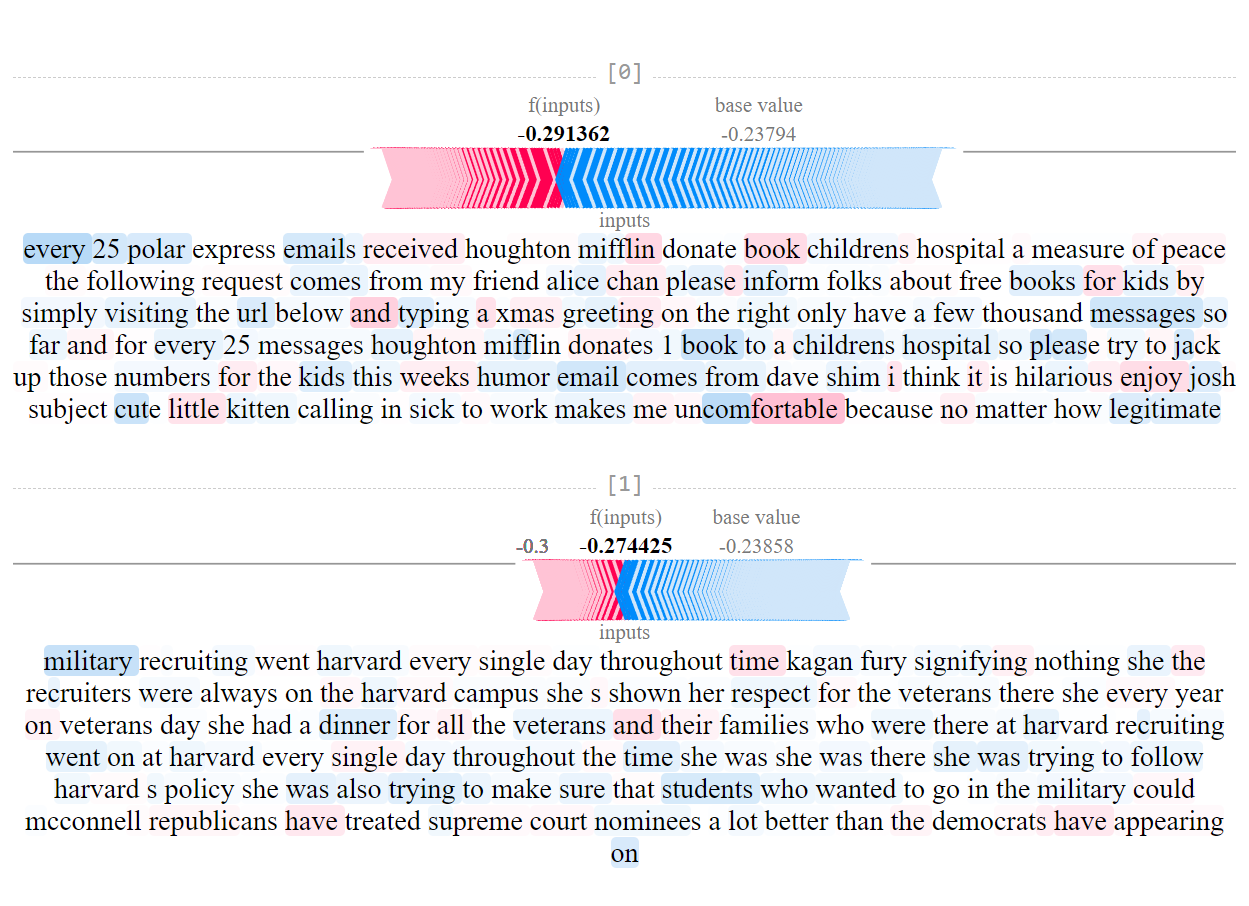
\includegraphics[width=\textwidth]{figs/one-distil-b-ml-c.png}
        % \caption{{DistilBERT}\textsubscript{B, C}}
    \endminipage\hfill % maximize horizontal separation
    \minipage{0.32\textwidth}
        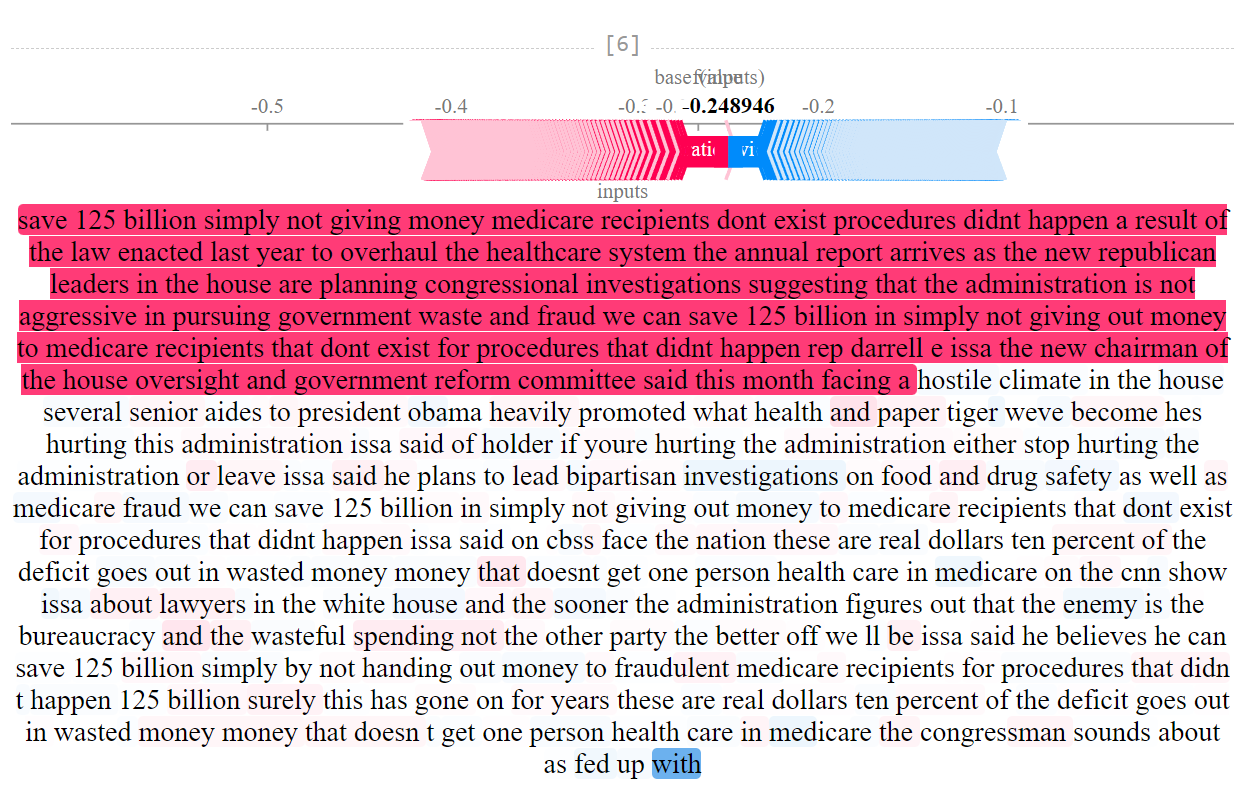
\includegraphics[width=\textwidth]{figs/all-distil-b-ml-c.png}
        % \caption{{DistilBERT}\textsubscript{B, C}}
    \endminipage\hfill % maximize horizontal separation
    \minipage{0.32\textwidth}
        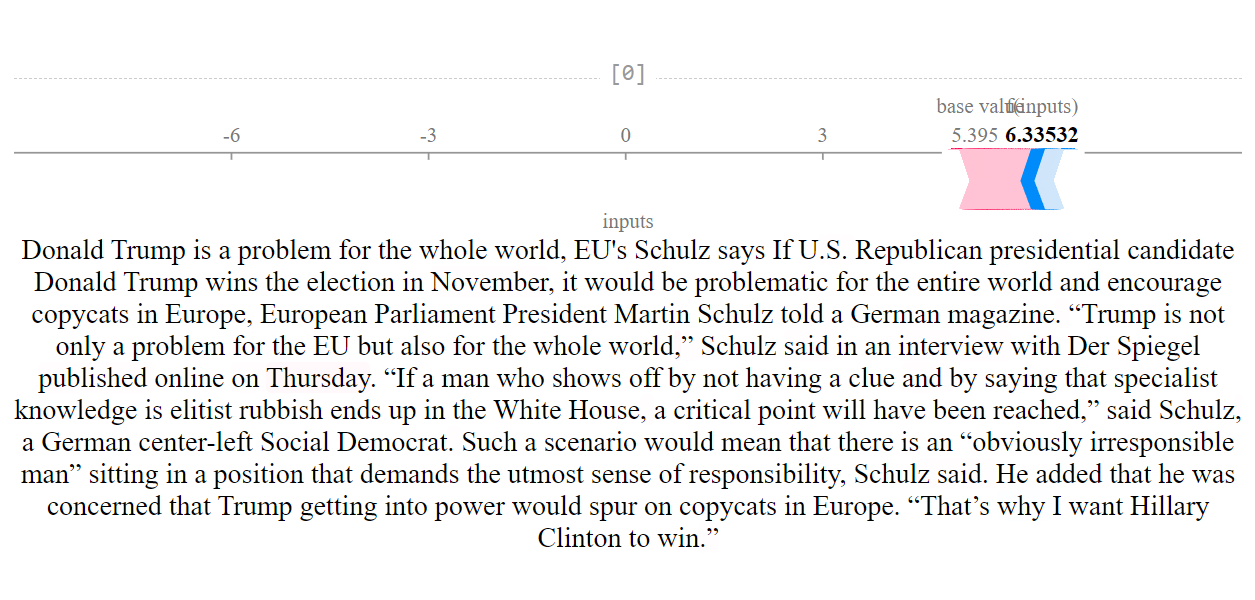
\includegraphics[width=\linewidth]{figs/news-distil-b-ml-c.png}
        % \caption{{DistilBERT}\textsubscript{B, C, ML}}
    \endminipage
    
    \caption{Valores Shapley de {DistilBERT}\textsubscript{B, C, ML} para los tres \textit{datasets}.}
    % \label{fig:shap-ps-one}
\end{figure}

\begin{itemize}
    \item LARGE, CASED, ML \textit{vs.} otros\footnote{Existen algunas excepciones según \textit{dataset} y modelo}.
    \item Rendimiento general: {P-S}\textsubscript{All} $>$ {P-S}\textsubscript{One} $>$ {News}.
\end{itemize}

\end{frame}

\begin{frame}{5.7. Evaluación}
\begin{itemize}
    \item LARGE ofrece resultados más consistentes.
    \item Alto valor de \textit{specificity}: gran capacidad de detectar noticias verdaderas.
    \item Análisis cuantitativo \textit{vs.} cualitativo: resultados generalmente poco concluyentes; distinto a lo esperado (\textit{datasets}, modelos...).
\end{itemize}
    
\end{frame}

\section{Discusión}
\begin{frame}{6. Discusión}

\begin{itemize}
    \item SHAP: limitaciones en la interpretación (alta variabilidad, escasa justificación matemática, etc.).
    \item Limitaciones de los modelos BERT: conocimiento sintáctico, semántico, sentido común, etc.
    \item Posibles sesgos:
    \begin{itemize}
        \item \textit{Word Embeddings}: sesgos implícitos, diferencia de criterios estático \textit{vs.} contextuales.
        \item Tokenización: \textit{cased} \textit{vs.} \textit{uncased}.
        \item Destilado de modelos: $\uparrow$ sesgos, no relacionado con tamaño del modelo.
        \item Modelos aumentados: mayor capacidad de adquirir sesgos.
    \end{itemize}
\end{itemize}

\end{frame}

\section{Conclusiones}
\begin{frame}{7. Conclusiones}

Objetivos propuestos y grado de cumplimiento:
\begin{itemize}
    \item Definir \textit{fake news}, delimitar área de estudio.
    \item Desarrollar un clasificador de \textit{fake news}.
    \item Estudio comparativo de rendimiento: \textit{datasets}, modelos.
    \item Estudio del rendimiento con XAI.
    \item Estudiar los sesgos involucrados en el estudio.
\end{itemize}

\end{frame}

% \section{Trabajos futuros}
% % \begin{frame}{Trabajos futuros}
    
% \end{frame}

\section*{Bibliografía}
\begin{frame}[noframenumbering,plain,allowframebreaks]{Referencias}
        \printbibliography
\end{frame}

\end{document}

